\section{Quick start}
\label{sec:quickstart}

\subsection{A first scan, on the simulated rack}

\begin{enumerate}
    \item Launch \oracle{}. On \app{Scan controls}, tick the first range and set
        \app{From (V)} 15 and \app{To (V)} 85, \app{Stepsize (V)} 1, \app{Bunches per
        channel} 25 and \app{Scan type} Sawtooth.
    \item Press \app{Start scan}. \oracle{} calibrates the scan's own setpoints, puts the
        calibration through the gate, writes the run's header and starts. The plots fill
        as hits arrive (Figure~\ref{fig:scan}); the simulated beam has lines at 32, 47 and
        71\,V.
    \item Press \app{Stop after scan} to end at the end of the scan in progress, or
        \app{Stop now!} to end within a bunch.
    \item The run is analysed as it closes: \app{Scan Performance} gives its verdict, and
        \app{Scan Calibration} its calibration.
    \item \menu{File > Open run...} (Ctrl+O, Cmd+O on macOS) brings any run back as it was
        taken.
\end{enumerate}

\begin{figure}[ht]
    \centering
    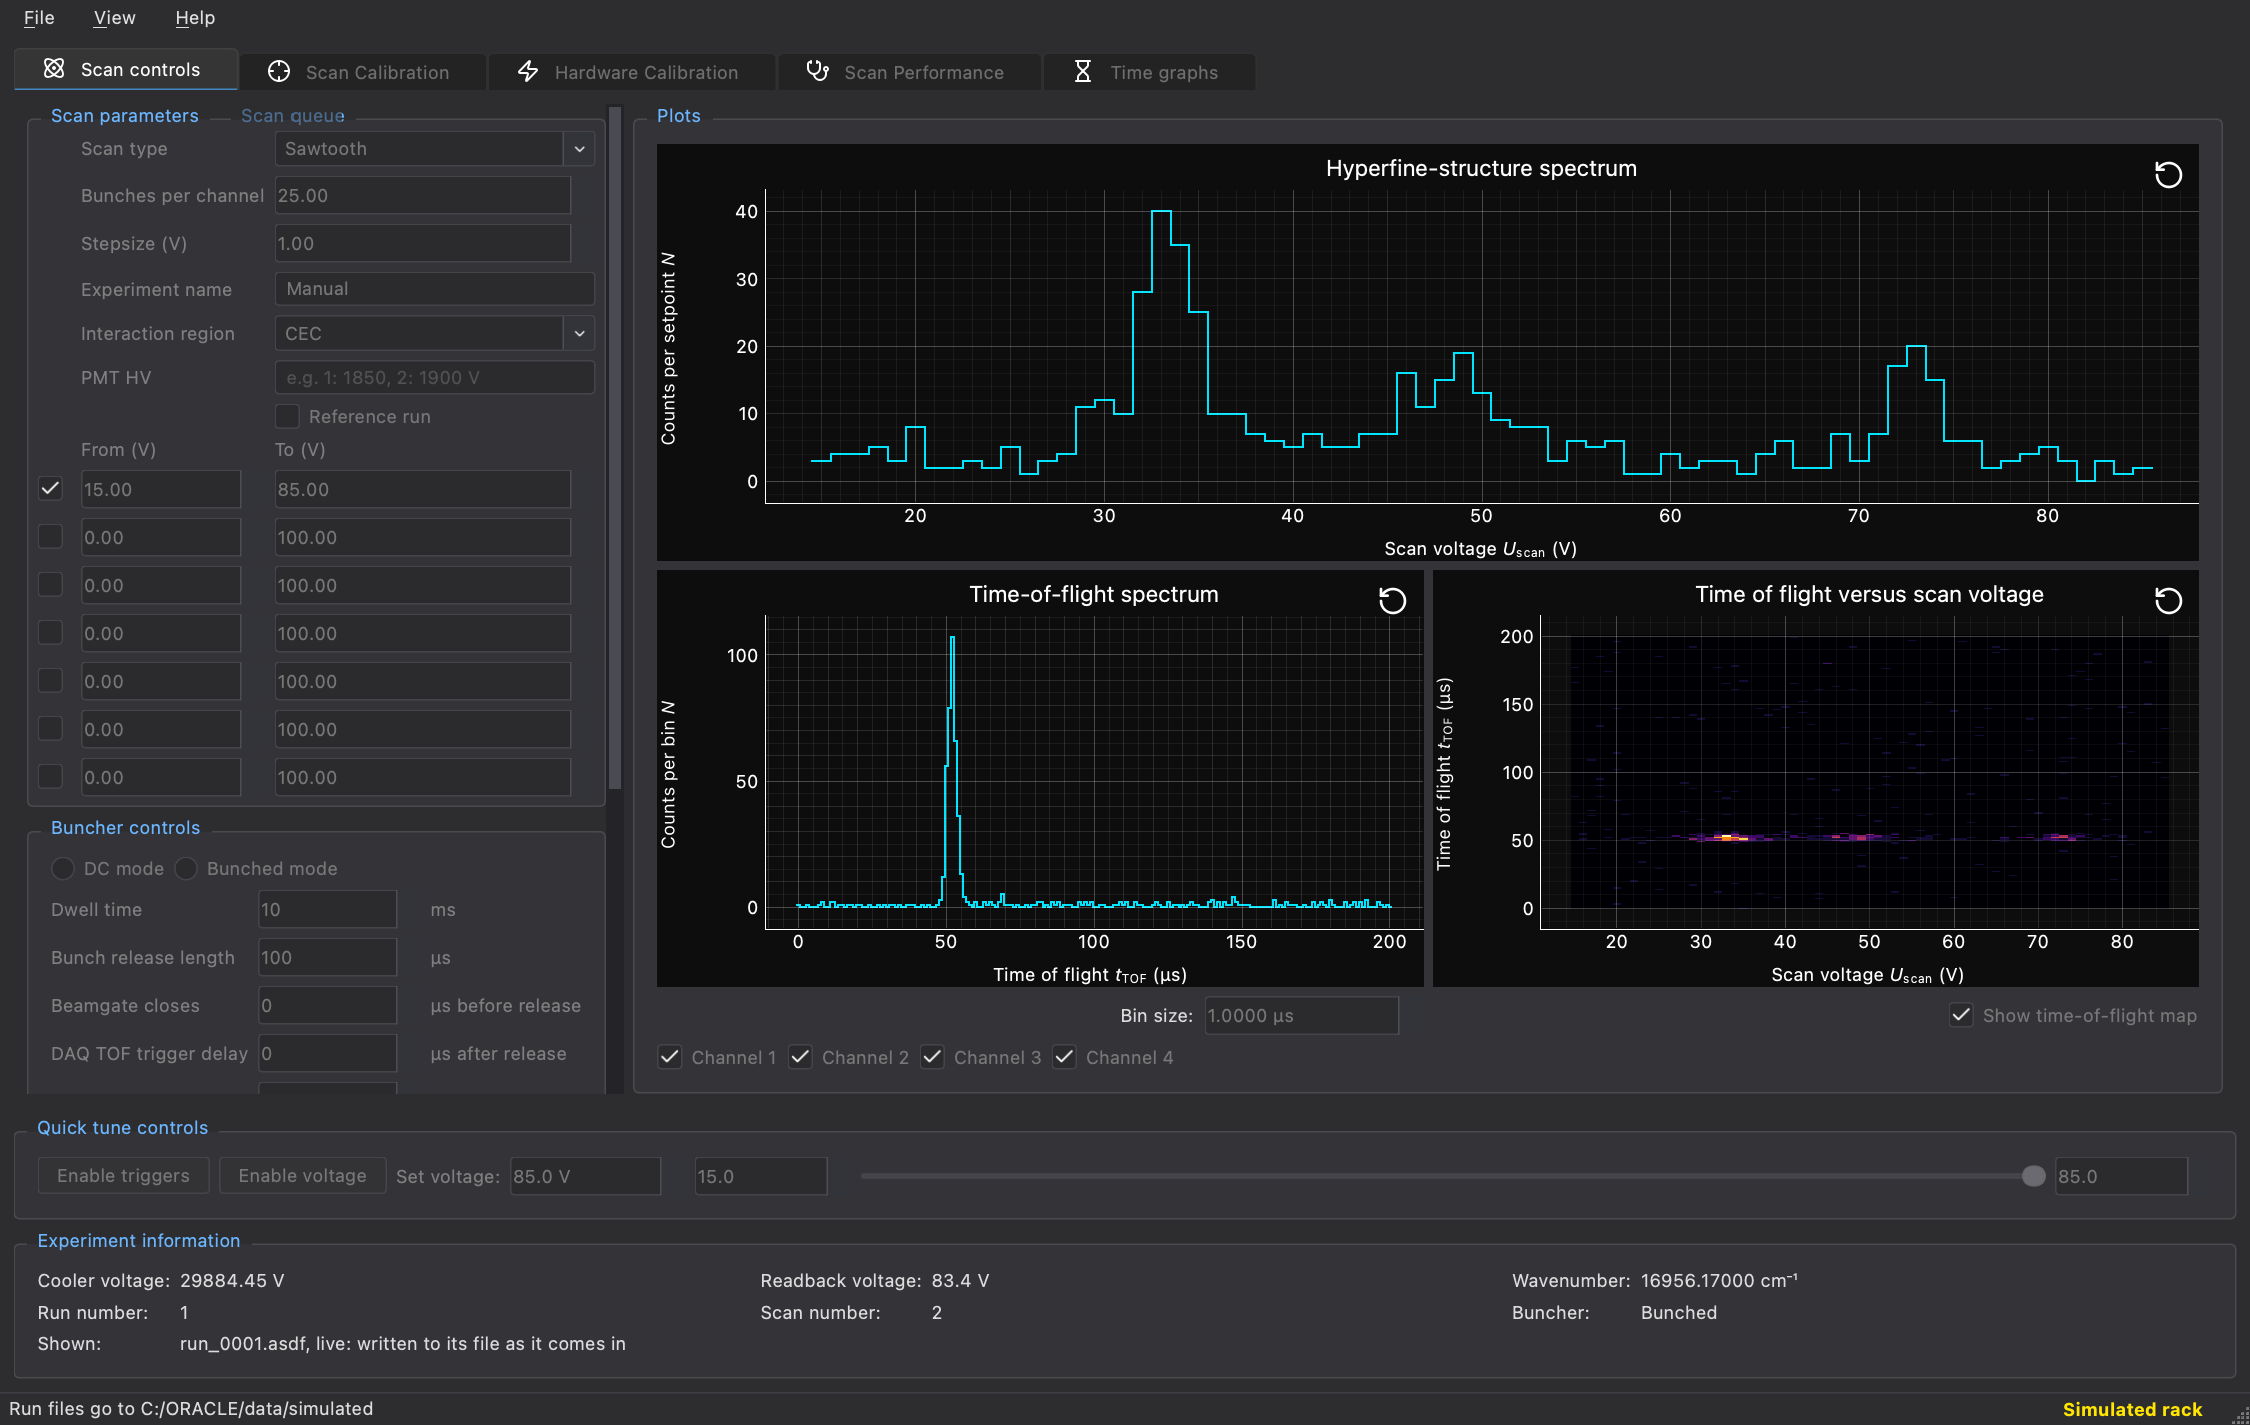
\includegraphics[width=\textwidth]{fig_scan_tab}
    \caption{The \app{Scan controls} tab during a simulated scan: parameters on the left,
        the hyperfine-structure spectrum, time-of-flight spectrum and map on the right,
        quick tune and the experiment information below.}
    \label{fig:scan}
\end{figure}

\subsection{A shift on the beamline}

\begin{enumerate}
    \item Read the status bar. A rack warning (a fault \oracle{} cannot mend, or hardware
        changed since the last session) is named there, its sentence in the tooltip.
    \item Run the \app{Health check} (\app{Hardware Calibration}), with \app{Check the bench
        table first} ticked: the table, the cooler's ripple, each PMT's dark counts, the
        triggers and both meters' trigger sources, set against the last check.
    \item If the hardware changed, measure the settle model (\app{Settle time}) and the
        bench table (\app{Scan table}) again before taking data.
    \item On \app{Scan controls}, set the \app{Experiment name}, the \app{Interaction region}
        and the \app{PMT HV}, and the buncher timing.
    \item Take scans one at a time, or lay them out in the \app{Scan queue} and let it run
        unattended.
    \item Read each run's \app{Scan Performance} verdict, and anything flagged for review,
        before fitting it in \denis{}.
\end{enumerate}
